% Chapter 2

\chapter{Introducción a las antenas polarimétricas y sus problemas} % Chapter title
\label{ch:phasedArray}
\lhead{\emph{Introducción a las antenas polarimétricas y sus problemas}}
%----------------------------------------------------------------------------------------

\section{Antenas polarimétricas}

Una antena polarimétrica es una antena que se la utiliza en radares y satélites. Generalmente trabajan en la
zona del espectro electromagnético de microondas. Las mismas pueden ser activas o pasivas, esto es, para el
primer caso, que el sistema emita su propia energía, para luego medir el eco de la misma. Para el segundo caso,
el radar no emite ninguna señal, simplemente recibe el eco de algún otro sistema emisor/receptor.

\begin{figure}[H]
 \centering
 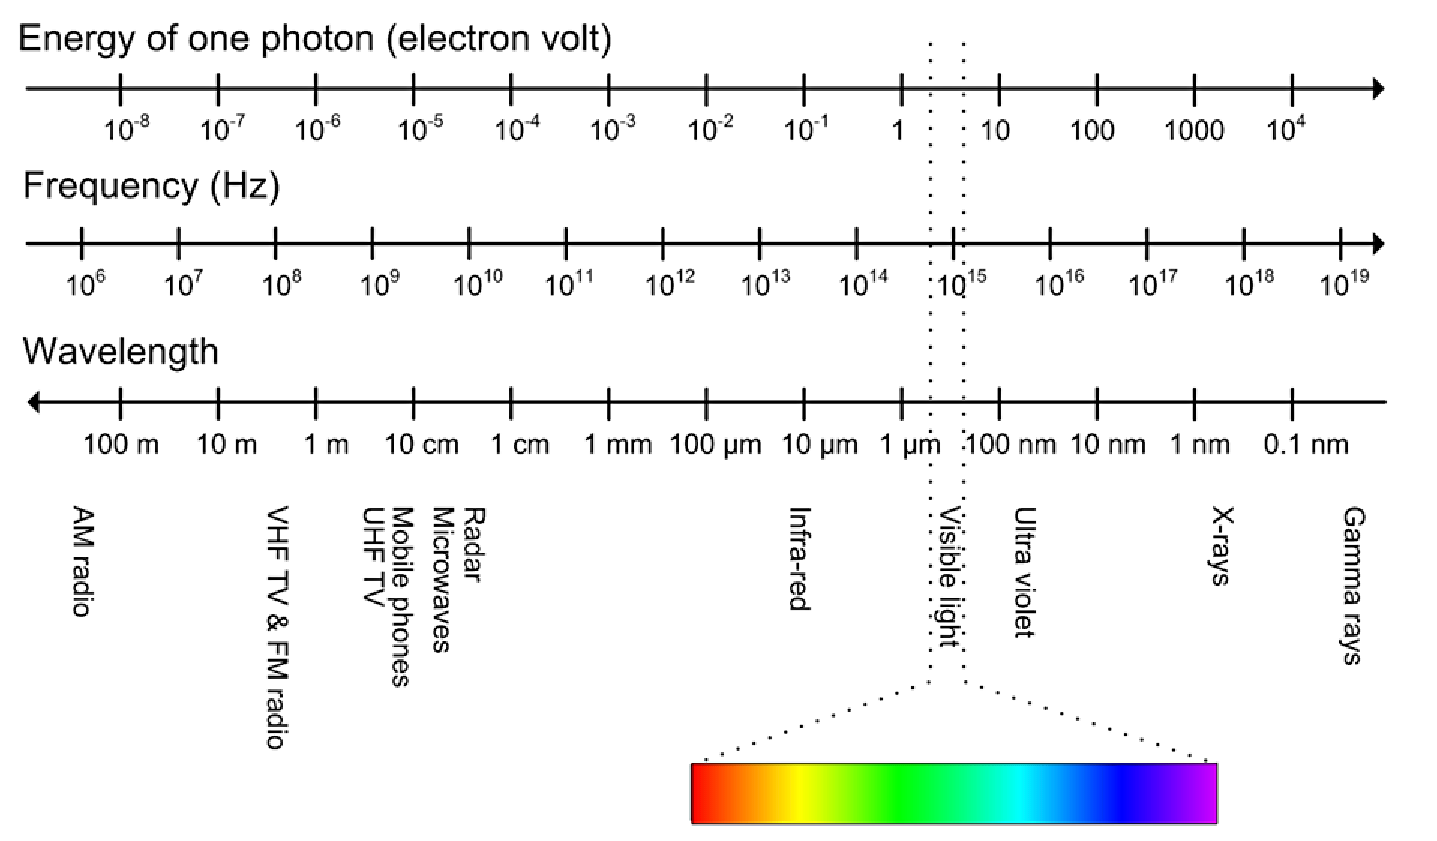
\includegraphics[width=10cm]{gfx/electromagneticSpectrum.png}
 \caption{Espectro Electromagnético \cite{electromagneticField}}
 \label{fig:spectrum}
\end{figure}


Dado que la frecuencia de trabajo está comprende la región microondas del espectro electromagnético, el cual está entre los 
300 MHz y los 300 GHz (ver figura \ref{fig:spectrum}), y dado que en dicho rango la opacidad de la atmósfera es casi nula 
(ver figura \ref{fig:atmosphere}), estas antenas poseen la capacidad de trabajar independientemente de las condiciones 
atmosféricas, esto es, que la señal casi no es atenuada por la atmósfera, tampoco es interferida ni por las lluvias ni por 
las nubes. A su vez, se puede obtener información sobre la textura del terreno y sobre los sustratos inferiores de las 
coberturas boscosas. Dependiendo de que longitud de onda del rango de trabajo, se tiene de 3 cm a 30 cm de penetración.

\begin{figure}[H]
 \centering
 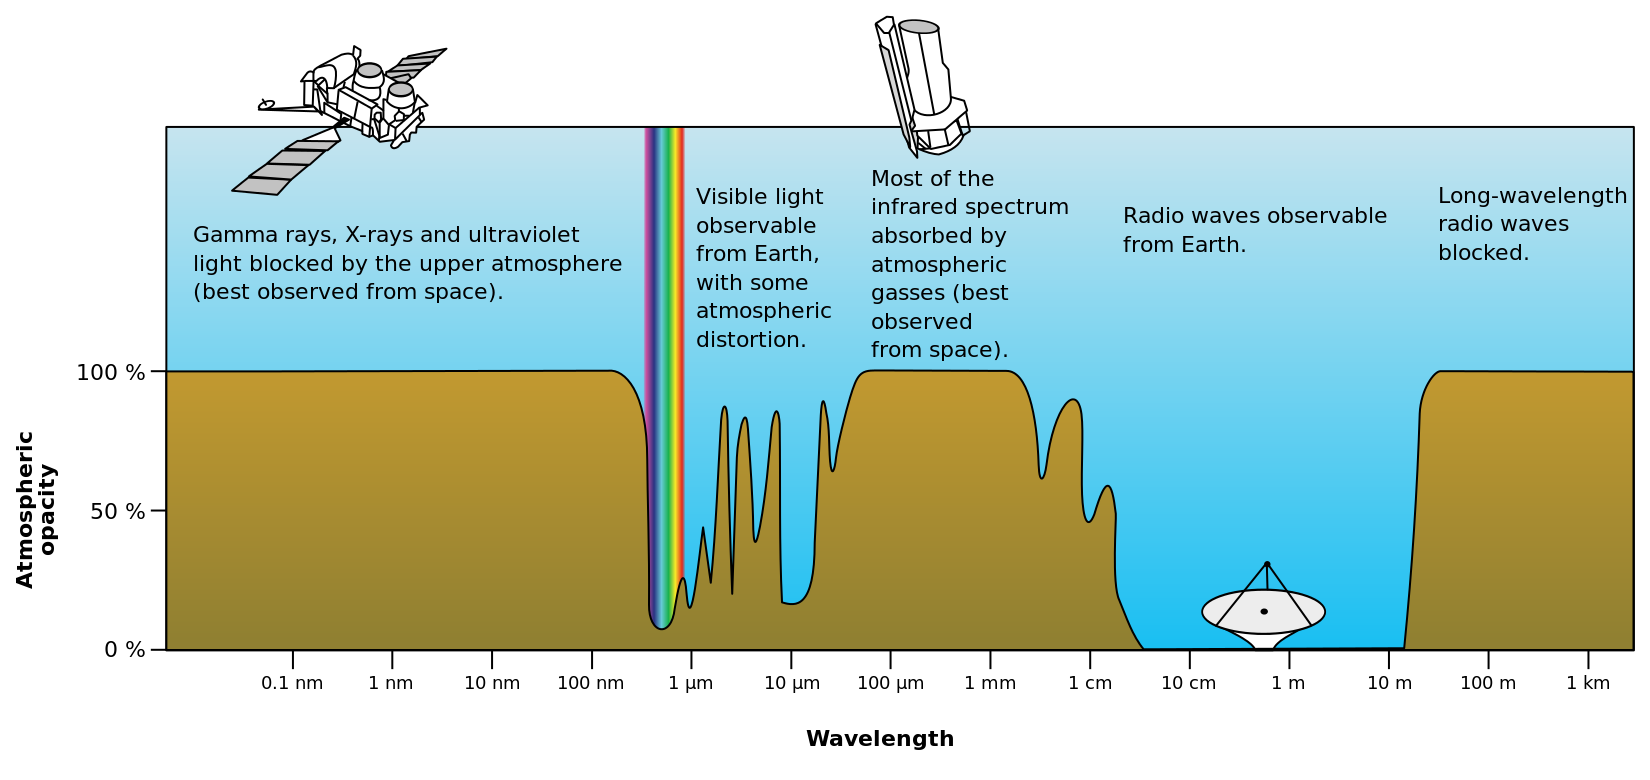
\includegraphics[width=10cm]{gfx/AtmosphericOpacity.png}
 \caption{Opacidad atmosférica vs longitud de onda \cite{electromagneticOpacity}}
 \label{fig:atmosphere}
\end{figure}

Por convención, el eje de referencia que es paralelo a la dirección del recorrido del satélite se lo llama azimuth. La
dirección del eje perpendicular, rango. El nadir es el punto más cercano de la tierra al satélite; en otras palabras, 
es el punto en la superficie terrestre que, si se trazara una recta perpendicular al mismo, también corta al satélite.

La antena nunca apunta diréctamente hacia abajo porque, de esta forma, se perdería mucha información en rango. Al apuntar 
en diagonal, y gracias a que el blanco no es puntual, el eco de la señal de la zona iluminada más cercana al nadir llega 
antes al satélite que la más alejada, logrando así, tomar muestras de distintos lugares espaciados en rango (ver figura 
\ref{fig:antena_ilumination}).

\begin{figure}[H]
 \centering
 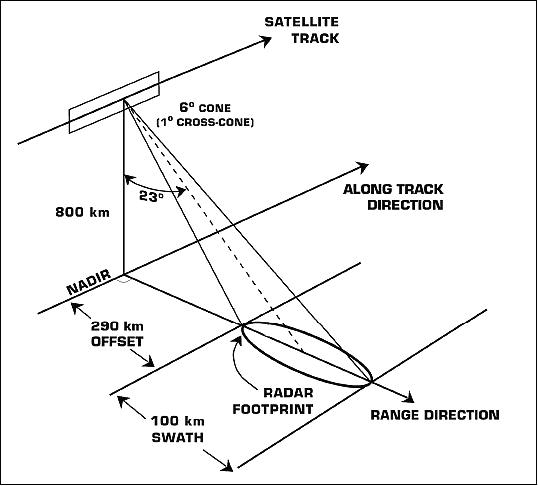
\includegraphics[width=7cm]{gfx/satellite.png}
 \caption{Footprint del satélite}
 \label{fig:antena_ilumination}
\end{figure}

El tamaño de la zona iluminada se llama footprint. Dicho tamaño depende tanto de las dimensiones de la antena como de la 
órbita del satélite o de la altura del avion en que está colocada dicha antena. Como se observa en la imagen 
\ref{fig:footprint}, mientras más larga es la antena, más angosto es el footprint, logrando así mejorar la resolución 
espacial.

\begin{figure}[H]
 \centering
 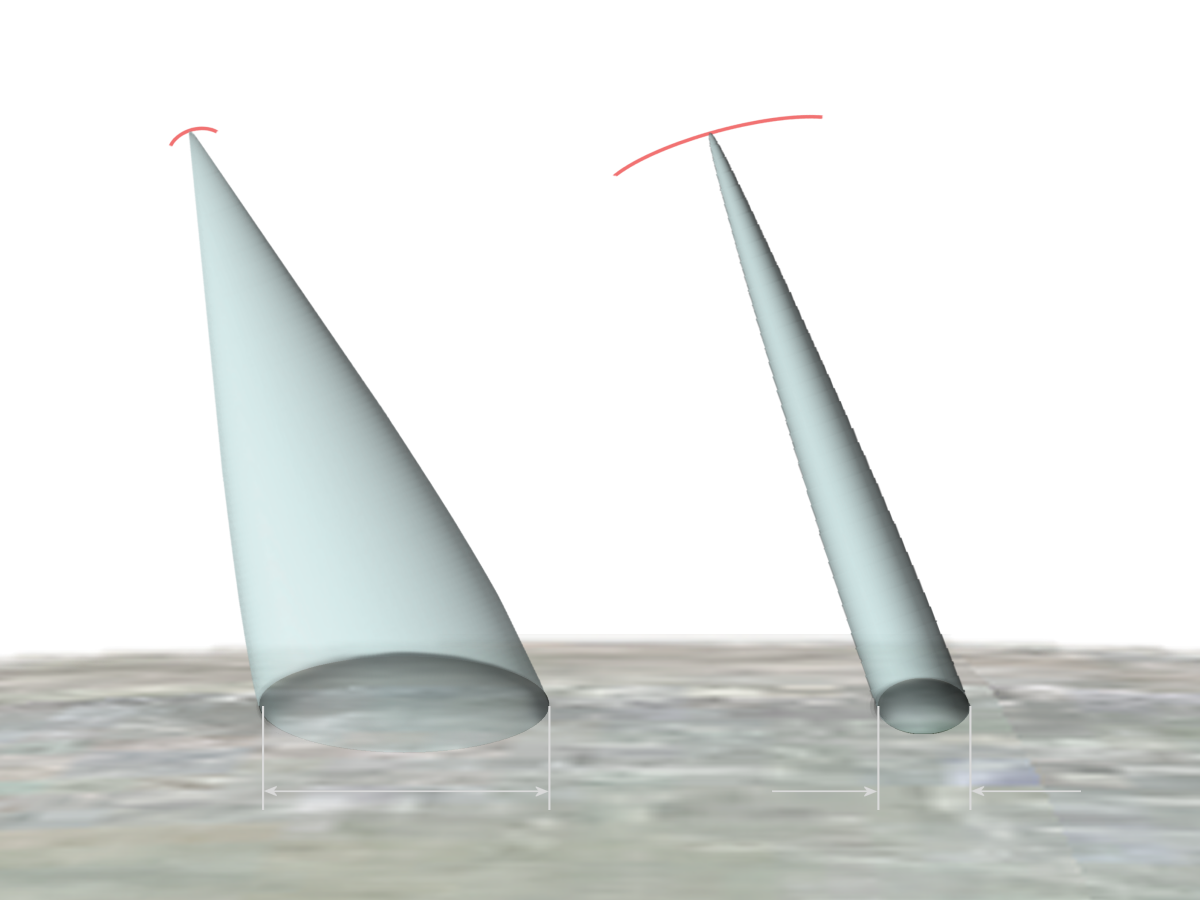
\includegraphics[width=7cm]{gfx/footprint.png}
 \caption{El footprint depende del largo de la antena}
 \label{fig:footprint}
\end{figure}

\subsection{Composición de una antena}

Un conjunto de de una antena polarimétrica es una colección de N módulos radiantes espaciados. Todos los elementos poseen los
mismos diagramas de radiación y están orientados en el mismo sentido y dirección en un ambiente tridimensional. No es 
necesario que los elementos estén espaciados regularmente ni que emitan los mismos valores de potencia y fase, pero se asume 
que todos están alimentados con la misma frecuencia de trabajo. En la figura \ref{fig:phasedArrayAntenna} se pueden observar
dos tipos de distribuciones comunmente utilizadas.

\begin{figure}[H]
	\centering
 	\subfloat[]{
		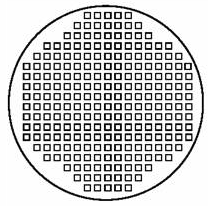
\includegraphics[width=4cm]{gfx/phasedArrayAntenna.png}}
	\subfloat[]{
		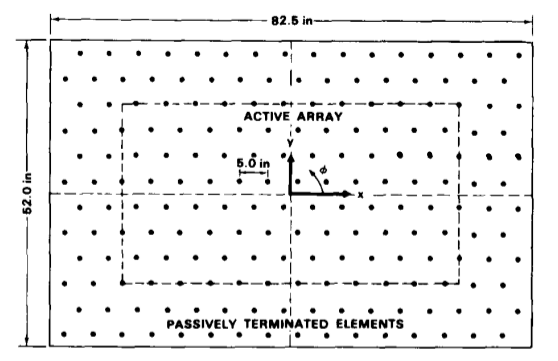
\includegraphics[width=6cm]{gfx/frontAntenna.png}}
	\caption{ (a) Conjunto de antena circular. (b) Conjunto de antena rectangular}
	\label{fig:phasedArrayAntenna}
\end{figure}

Este tipo de antenas están compuestas por tres bloques principales; los cuales son el generador, la red de distribución (o RFDN) y la 
antena con los módulos radiantes (ver figura \ref{fig:compositionAntenna}).

\begin{figure}[H]
 \centering
 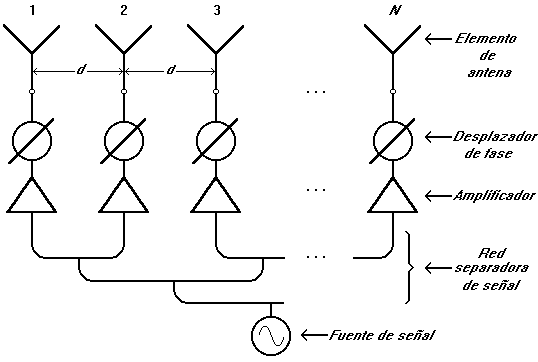
\includegraphics[width=10cm]{gfx/CompositionAntenna.png}
 \caption{Composición de un conjunto de antena}
 \label{fig:compositionAntenna}
\end{figure}

El generador de puede emitir distitnos tipos de modulaciones. Ej, cuadrada, chirp, senoidal, triangular, etc. Las ventajas y
desventajas de cada una se lista en el cuadro \ref{tab:modulations}

\begin{table}[H]
  \footnotesize
  \centering
  \begin{tabular}{|c|p{9cm}|}
	\hline
	\textbf{Modulación} & \textbf{Cacarcterísticas} \\
	Cuadrada & Esta modulación es utilizada para mediciones muy precisas a cortas distancias comparando las fases de los dos 
	semiciclos de la señal recibida. La desventaja es que los distintos ecos de los distintos blancos no pueden distinguirse.\\\hline
	Chirp & Es la modulación mayormente utilizada, se obtienen mediciones con las mayores distancias posibles.\\\hline
	Triangular & Con esta modulación se logra distinguir fácilmente la velocidad de la posición del blanco. \\\hline
	Escalonada & Es utilizada para mediciones de interferometría y para expandir el rango de medición sin ambig\"uedades.\\\hline
  \end{tabular}
  \caption{Cacacterísticas de cada modulación de la señal emitida}
  \label{tab:modulations}
\end{table}

La red de distribución, llamada RFDN, es la encargada de transmitir la señal a todos los módulos radiantes de la antena. 
Dicha red posee una estructura de árbol, de forma tal, que la longitud de todos los caminos entre las hojas del mismo a 
la raíz son iguale (Los nodos son los PSC y las holas los RMs). Es necesraio que todos los caminos sean iguales para que la 
señal transmitida posea la misma fase y atenuación. Los componentes utilizados para distribuir la señal son los siguientes:

\begin{itemize}
	\item Power Splitter Combiner: este componente es el encargado de dividir la señal transmitida en tantos puertos de salida 
		tenga y la de sumar/combinar las potencias recibidas.
	\item Cable: este componente es el utilizado para unir el resto de los componentes.
	\item Módulo de Transmisión y Recepción: Este componente es el encargado de atenuar y amplificar la señal para que, tanto
		la potencia transmitida como la entrante a la red esté controlada y conocida. Hay uno por cada módulo radiante para 
		poder calibrar la antena, esto es, que la potencia de salida/entrada sea la misma en cada módulo radiante.
	\item Defasador: Este componente simplemente defasa la señal transmitida, hay uno por cada módulo radiante, se lo utiliza
		para poder calibrar la antena tanto en transmisión como en recepción, logrando así, que cada camino de transmisión/
		recepción de las hojas a la raíz defase lo mismo. A su vez, se lo utiliza para poder direccionar el beam de la señal
		emitida.
	\item Módulo Radiante: Este componente es el emisor de la señal a transmitir y/o el receptor. En este tipo de antenas un 
		RM puede cumplir una o ambas funcionalidades.
	\item Circulador: Este componente generalmente es uno de tres puertos, se lo utiliza para separar los caminos de la 
		señal transmitida (Tx) de la recibida (Rx). Generalmente es utilizado si el mismo módulo radiante se lo utiliza para
		transmisión como recepción.
\end{itemize}

Se pueden armar los módulos de tal forma que puedan transmitir en dos polarizaciones distintas, H y V (Ver figura 
\ref{fig:polarizations}), para esto, se debe duplicar la RFDN. Haciendo uso de ambas polarizaciones se puede caracterizar 
los blancos observados, dado que, cada cuerpo responde de forma distinta a cada tipo de polarización.

\begin{figure}[H]
 \centering
 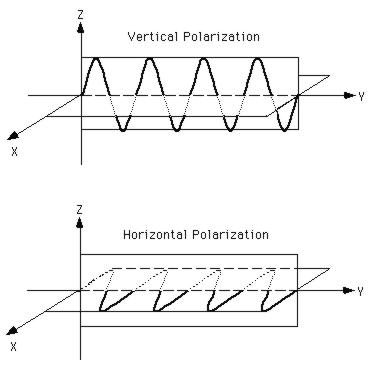
\includegraphics[width=7cm]{gfx/HAndVPolarizations.png}
 \caption{Polarizaciones verticales y horizontales}
 \label{fig:polarizations}
\end{figure}



\subsection{Diagrama de radiación de antena}

Un conjunto de antena puede armarse recursivamente, esto es, que un elemento sea, en si mismo, un conjunto. Un diagrama de antena es 
un diagrama de radiación polar que resulta de reemplazar cada elemento por un radiador isotrópico. Si se asume que el diagrama de
radiación de cada elemento es idéntico al del resto, tomando una cierta incertidumbre, el diagrama de radiación total resulta de
la multiplicación de todos los diagramas de todos los elementos. Este resultado no depende de si se consideran los diagramas de
potencia o de amplitud/fase.

\begin{figure}[H]
 \centering
 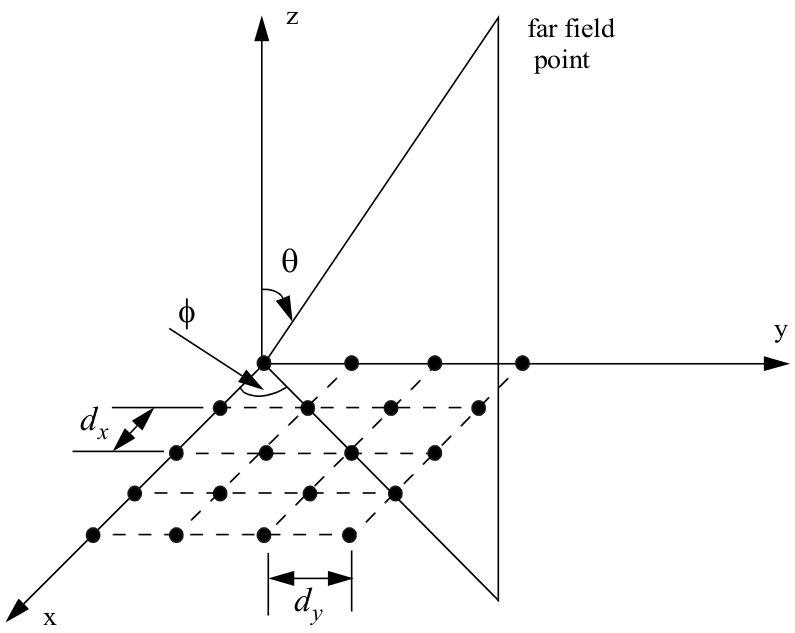
\includegraphics[width=7cm]{gfx/rectangularArrayGeometry.png}
 \caption{Conjunto de geometría rectangular \cite{Mahafza2004}}
 \label{fig:arrayGeometry}
\end{figure}

Considerese un conjunto de antena de $NxM$ elementos, como se muestra en la figura \ref{fig:arrayGeometry}, el diagrama de 
radiación de campo lejano se lo calcula de la siguiente forma \cite{Mahafza2004}.

\begin{equation}
	E(\theta, \phi) = \sum_{n=0}^{N-1}\sum_{m=0}^{M-1} I_{n,m} e^{jk(d_xn\sin\phi\cos\theta + d_ym\sin\phi\sin\theta)}
\end{equation}

Donde $\theta$ corresponde al ángulo al eje x, $\phi$ corresponde al ángulo al eje z, $k$ es el número de onda y es igual 
a $2\pi/\lambda$, $I_{n,m}$ es la amplitud compleja del elemento n,m. La figura \ref{fig:arrayPattern} muestra el diagrama de 
radiación en 3D, donde el eje $Z$ (representado con colores) es la potencia radiada. A su vez, se puede apreciar uno de los 
cortes que se realizan generalmente sobre los mismos (elevacion o azimuth).

\begin{figure}[H]
 \centering
	\subfloat[]{
		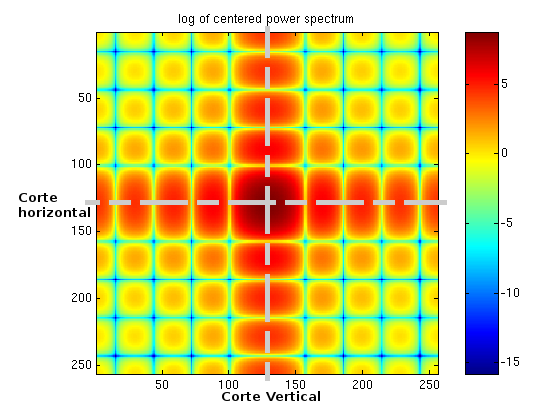
\includegraphics[width=7cm]{gfx/arrayPattern3D.png}}
 	\subfloat[]{
		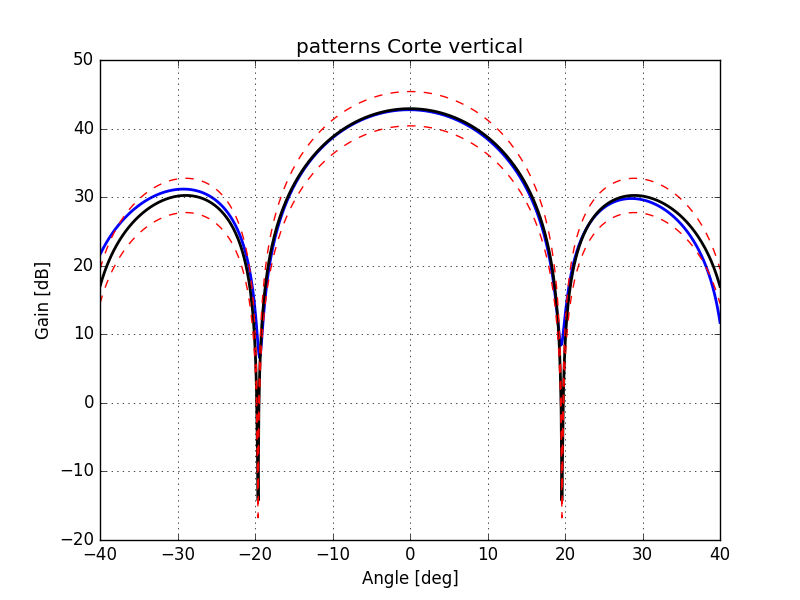
\includegraphics[width=7cm]{gfx/arrayPatternCut.png}}
	\caption{diagramas de radiación de un conjunto de antena (a) diagrama en 3 dimensiones \cite{arrayPattern} (b) corte horizontal}
 \label{fig:arrayPattern}
\end{figure}

A continuación se mostrarán gráficos representando la potencia del campo radiado, asumiendo campo lejano. La potencia decae 
con la relación de $1/r$, donde $r$ es la distancia del punto de medición al elemento radiado. Se debe tomar en cuenta también
la fase con que emite el elemento y el retardo de fase que se debe al tiempo en que tarda en llegar la señal a los distintos 
lugares del espacio. El retardo es expresado como $2\pi r/\lambda$, siendo $\lambda$ la longitud de onda de la señal emitida 
por el elemento radiado. Los gráficos \ref{fig:twoArrayPat} y \ref{fig:fourArrayPat} muestran las curvas de nivel de diagramas 
de radiación de pontencia polar. La separación de los módulos radiantes está en el eje x, eje horizontal y todos los elementos
están emitiendo en fase.

\begin{figure}[H]
	\centering
	\subfloat[]{
		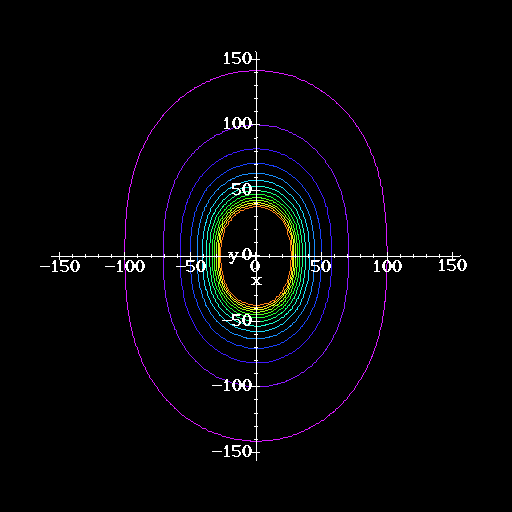
\includegraphics[width=5cm]{gfx/TwoIsoQuartDist.png}}
	\subfloat[]{
		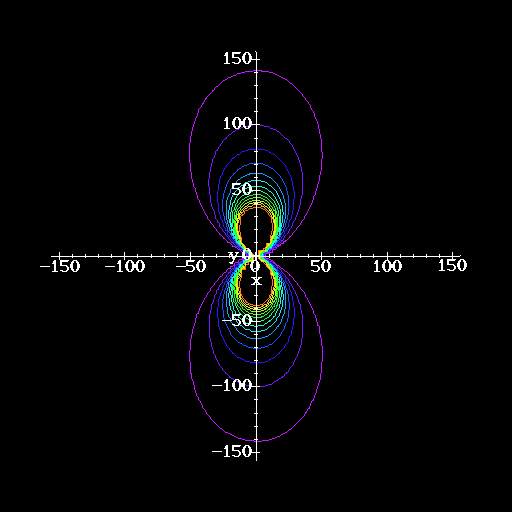
\includegraphics[width=5cm]{gfx/TwoIsoHalfDist.png}}
	\caption{Patrones de radiación de potencia. a) Dos elementos radiantes separados $1/4$ de longitud de onda, b)
	Dos elementos radiantes separados $1/2$ de longitud de onda}
	\label{fig:twoArrayPat}
\end{figure}

\begin{figure}[H]
	\centering
	\subfloat[]{	
		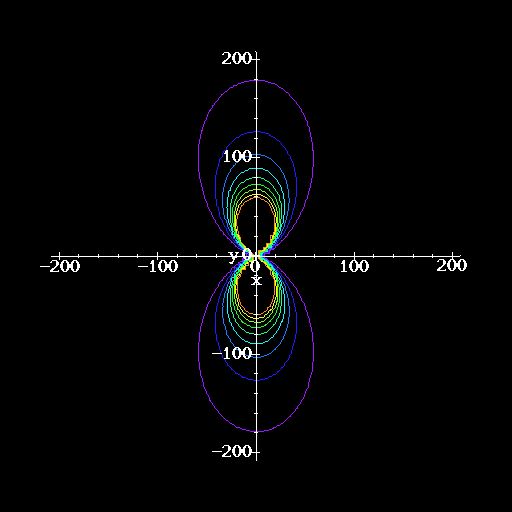
\includegraphics[width=5cm]{gfx/FourIsoQuartDist.png}}
	\subfloat[]{	
		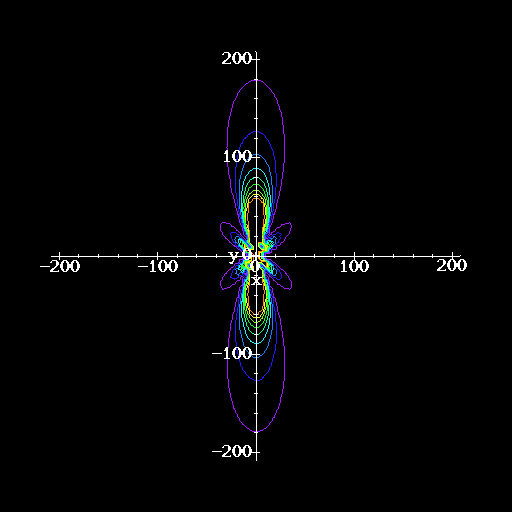
\includegraphics[width=5cm]{gfx/FourIsoHalfDist.png}}
	\caption{Patrones de radiación de potencia. a) Cuatro elementos radiantes separados $1/4$ de longitud de onda, b)
	Cuatro elementos radiantes separados $1/2$ de longitud de onda}
	\label{fig:fourArrayPat}
\end{figure}

Se puede observar que aumentando la cantidad de módulos radiantes, se logra que el beam principal (lóbulo principal de 
potencia), sea más angosto, por lo tanto se obtenga una mayor resolución del cuerpo observado. Observando la siguiente 
figura (\ref{fig:directArrayPat}), se puede deducir que la fase de los elementos radiados modifica la dirección del 
diagrama de radiación de antena.

\begin{figure}[H]
	\centering
	\subfloat[]{	
		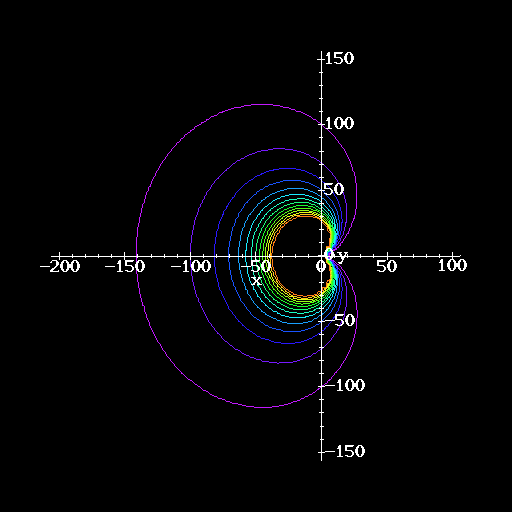
\includegraphics[width=5cm]{gfx/TwoQuarterPhase.png}}
	\subfloat[]{	
		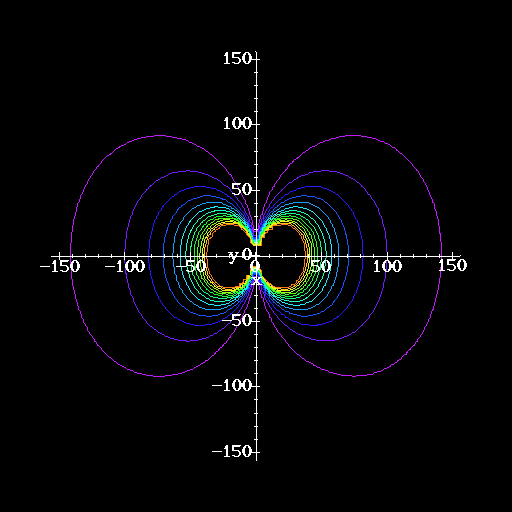
\includegraphics[width=5cm]{gfx/TwoAntiPhase.png}}
	\caption{Patrones de radiación de potencia. a) Dos elementos radiantes separados $1/4$ de longitud de onda y con 
		defasaje de $\pi$, b) Dos elementos radiantes separados $1/2$ de longitud de onda y en contrafase}
	\label{fig:directArrayPat}
\end{figure}

Directividad, el ancho del lóbulo principal, y el nivel de los lóbulos secundarios son los tres parámetros más importantes 
de un conjunto de antena \cite{Hsiao1985}.

Lamentablemente los errores del conjunto limitan los niveles que se pueden obtener de los lóbulos secundarios \cite{Hsiao1985}.

Como es bien sabido, si se achican los lóbulos secundarios, tanto la directividad como el ancho del lóbulo principal son
afectados. Para mantener ambas características invariantes, es necesario incrementar el tamaño del conjunto de antena 
\cite{Hsiao1985}.


\subsection{Apuntamiento de una antena}\label{ssec:beamSteering}

Para que la suma de todas las señales emitidas con todos los elementos radiantes apunte a un mismo punto, es necesario que 
todas las ondas lleguen al objetivo con la misma fase. Es por esto que se debe saber determinar cual es la fase individual que 
debe tener cada uno de los elementos radiantes. 

Como primer simplificación, se puede asumir que todas las rectas de cada uno de los elementos radiantes al punto lejano son 
paralelas entre ellas. A su vez, como el camino recorrido desde cada elemento radiante al punto lejano es diferente, es 
necesario calcular dicha diferencia para luego relacionarla con la fase. De esta forma, se puede retrasar la fase emitida de 
los elementos más alejados al punto para que todas las señales lleguen en fase, logrando así, una onda plana.

La figura \ref{fig:beamSteering} muestra como se realiza el apuntamiento de un conjunto de antena en una sola dirección,
para la dirección perpendicular, el razonamiento es totalmente análogo.

\begin{figure}[H]
 \centering
 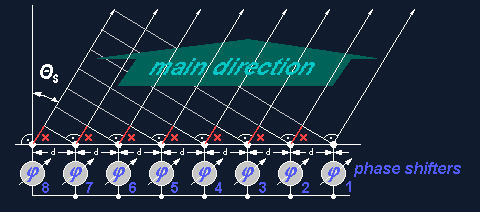
\includegraphics[width=10cm]{gfx/beamSteering.png}
 \caption{Apuntamiento con una conjunto de antena \cite{BeamSteering}.}
 \label{fig:beamSteering}
\end{figure}

Como se puede observar en la figura \ref{fig:beamSteering}, la diferencia de fase entre dos elementos consecutivos, 
$\Delta\varphi$, es constante y es llamada incremento de fase \cite{BeamSteering}. Se la puede relacionar con la diferencia 
de distancia que tiene que recorrer el haz emitido por cada elemento radiante. Dicha diferencia de distancia se la calcula con 
la siugiente relación matemática, 


\begin{equation}
	x = d\cdot \sin{\theta_s}
	\label{eq:steering}
\end{equation}

Donde $d$ es la distancia entre dos módulos consecutivos y $\theta_s$ es el apuntamiento deseado del haz emitido. Para calcular
el defasaje de una onda en una cierta distancia $x$, se debe tener en cuenta que es dependiente de su longitud de onda. 

\begin{equation}
	\dfrac{2\pi}{\Delta\varphi} = \dfrac{\lambda}{x}
	\label{eq:dist2angle}
\end{equation}

Donde $\Delta\varphi$ es el incremento de fase entre módulos radiantes, $\lambda$ es la longitud de onda transmitida, 
Utilizando las ecuaciones \ref{eq:steering} en \ref{eq:dist2angle} se puede obtener el incremento de fase entre módulos radiantes
contiguos necesario para cumplir con el apuntamiento deseado. La ecuación matemática a continuación.

\begin{equation}
	\Delta\varphi = \dfrac{2\pi\cdot d\cdot\sin{\theta_s}}{\lambda}
\end{equation}

\subsection{Calibración interna de una antena polarimétrica}

No solo la respuesta de los componentes varía por el envejecimiento de los mismos al pasar del tiempo, haciendo que dejen de
comportarse de forma nominal, sino que, también lo hacen a causa de variaciones en la temperatura de operación, que hayan sido
utilizados de forma imprudente, por interferencias electromagnéticas (radiadas o conducidas), etc. Es por esta razón que se 
tienen que corregir dichas variaciones, buscando que no solo todos los caminos de recepción atenúen y defasen exactamente lo
mismo, sino que también sea un valor conocido. En transmisión el objetivo es el mismo, con la salvedad que se busca que cada 
TRM trabaje en su punto de compresión (generalmente cerca de los 6dB) y la fase de cada elemento depende del apuntamiento 
deseado. 

Para calibrar la antena por medio de lazos de calibración, la electrónica central es como un VNA (representado en la figura 
\ref{fig:calibrationLoop}). La misma emite una señal por un canal y la compara con lo recibido por el otro canal, midiendo el 
S21 (transmisión directa) de los parámetros S de la antena.

\begin{figure}[H]
 \centering
 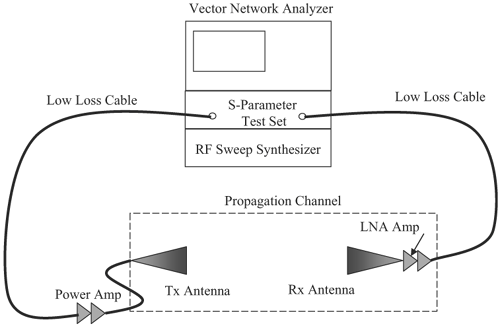
\includegraphics[width=10cm]{gfx/calibrationLoop.png}
 \caption{Lazo de calibración utilizando un VNA.} 
 \label{fig:calibrationLoop}
\end{figure}

La figura \ref{fig:nonCalPattern} muestra la comparación de dos diagramas de radiación de antena, uno calibrado e ideal y el 
otro sin calibrar. Se puede observar como los niveles de los lóbulos secundarios y el ancho del lóbulo principal se incrementa.

\begin{figure}[H]
 \centering
 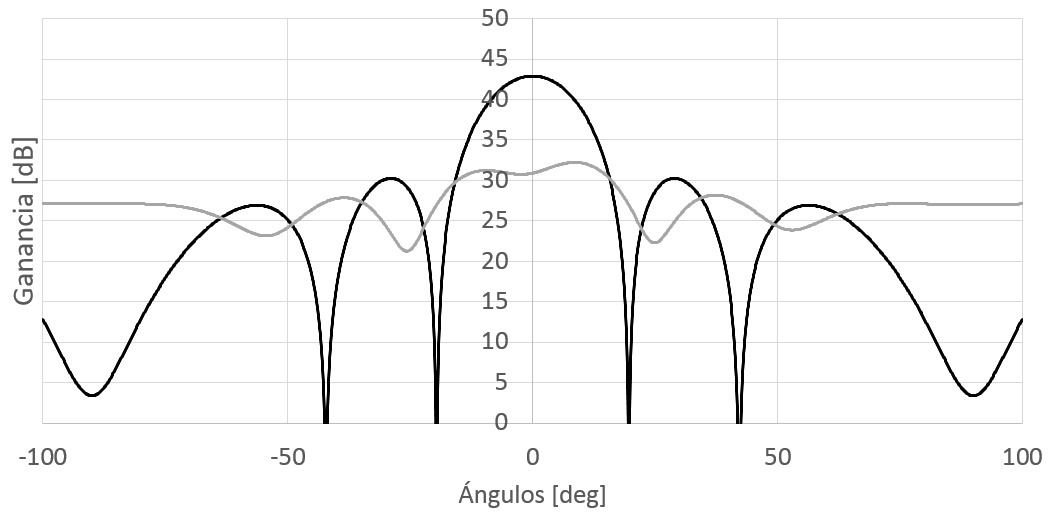
\includegraphics[width=10cm]{gfx/nonCalPattern.png}
 \caption{Diagrama de radiación de antena calibrado vs no calibrado.}
 \label{fig:nonCalPattern}
\end{figure}

\section{Parámetros S}

La sigla S deriva de la palabra scattering. Para altas frecuencias, es conveniente describir una
determinada red en términos de ondas en vez de tensiones o corrientes. Esto permite una definición más 
sencilla de planos de referencia. Por razones prácticas, la descripción en términos de ondas entrantes
y salientes ha sido introducida. Ahora, una red de 4 polos se transforma en 2 puertos y $2n$ polos se 
transforman en $n$ puertos. En el caso de un número impar de polos (ej. 3 polos), un punto de referencia
puede ser elegido, atribuyendo un polo igualmente a dos puertos. Por lo tanto 3 polos se convierten en 
3 + 1 polo correspidiendo a 2 puertos. Como una regla general, para cantidades impares de polos, siempre
se agrega un polo extra.

\begin{figure}[H]
 \centering
 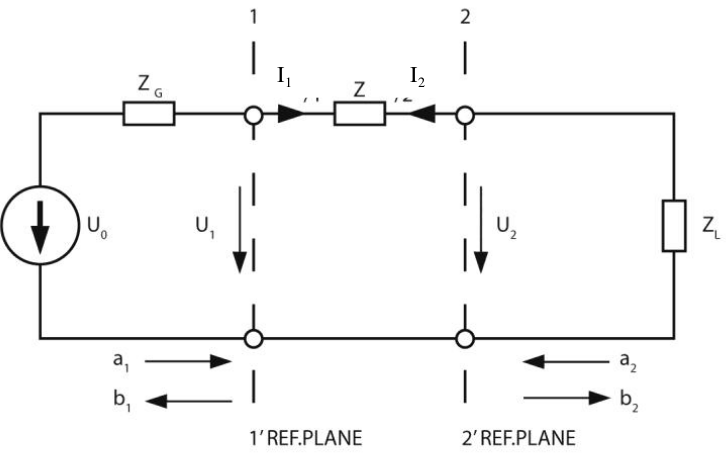
\includegraphics[width=10cm]{gfx/sParameters1.png}
 \caption{Ejemplo de una red de 2 puertos: circuito serie}
 \label{fig:esquema_serie}
\end{figure}

Tomando como ejemplo una red de 2 puertos compuesta por una sola impedancia $Z$ conectada en serie (\ref{fig:esquema_serie}).
Las impedancias de la fuente y de la carga son $Z_G$ y $Z_L$ respectivamente. Si $Z=0$ y $Z_L = Z_G$ (para el caso de $Z_G$ real) 
la carga está adaptada. En este caso se obtiene una máxima transferencia de potencia y $U_1 = U_2 = U_0/2$. Notar que todas las
tensiones y corrientes son valores pico. Se supone que las líneas que unen los componentes poseen longitud eléctrica igual a 0. 
Las conecciones con una longitud eléctrica finita están dibujadas como una doble líea. A continuación se relacionará $U_0$, $U_1$ 
y $U_2$ a $a$ y $b$.


\subsection{Definición de \enquote*{ondas de potencia}}

Las ondas incidentes al puerto son $\textbf{a}=(a_1, a_2, a_3, ..., a_n)$, las ondas salientes, o reflejadas, del puerto son  
$\textbf{b}=(b_1, b_2, b_3, ..., b_n)$. Por definición, las corrientes incidentes son positivas y las salientes negativas. La
onda $a_1$, incidente al puerto 1, es derivada de la tensión entrante a la carga balanceada. 

Para hacer qe esta definición sea consistente con la ley de la conservación de la energía. La tensión es normalizada a $\sqrt{Z_0}$. 
$Z_0$ es, en general una impedancia de referencia arbitraria, que usualmente se la utiliza como la impedancia característica de la 
línea (ej, $Z_0 = 50 \Omega$). Y, cuando todas las impedancias son iguales ($Z_G = Z_L = Z_0$), se dice que la línea está adaptada
y no hay onda reflejada. Las definiciones de $a1$ y $b1$ son:

\begin{equation}
\begin{aligned}
	a1 &= \dfrac{U_0}{2\sqrt{Z_0}}= \dfrac{\textrm{onda de tensión incidente (puerto 1)}}{\sqrt{Z_0}}=\dfrac{U_1^{inc}}{\sqrt{Z_0}} \\
	b1 &= \dfrac{U_1^{refl}}{2\sqrt{Z_0}}= \dfrac{\textrm{onda de tensión reflejada (puerto 1)}}{\sqrt{Z_0}}
\end{aligned}
\end{equation}

Notar que \textbf{a} y \textbf{b} tienen las unidades de $\sqrt{\textrm{potencia}}$.

La potencia incidente al puerto 1, $P_{inc}$, es simplemente la potencia entregada por la fuente, mientras que la potencia saliente 
del puerto 1, $P_{refl}$, viene de la onda de tensión reflejada.

\begin{equation}
\begin{aligned}
	P_1^{inc} &= \dfrac{1}{2}|a_1|^2= \dfrac{|U_1^{inc}|^2}{2Z_0}=\dfrac{|I_1^{inc}|^2}{2}Z_0 \\
	P_1^{refl} &= \dfrac{1}{2}|b_1|^2= \dfrac{|U_1^{refl}|^2}{2Z_0}=\dfrac{|I_1^{refl}|^2}{2}Z_0 \\
\end{aligned}
\end{equation}

En el caso de una desadaptación de la impedancia de carga $Z_L$, parte de la potencia será reflejada a través del puerto 2 (
potencia incidente al puerto 2).

$$
P_2^{inc}=\dfrac{1}{2}|a_2|^2
$$

Se ha definido $a_1 = U_0/2\sqrt{Z_0} = U^{inc}/\sqrt{Z_0}$ con la onda de tensión incidente $U^{inc}$. Como analogía 
se la puede definir como $a_1 = I^{inc}\sqrt{Z_0}$ con la onda incidente de corriente $I^{inc}$. Utilizando ambas, se obtiene la 
definición general de las ondas incidentes $a_i$ y reflejadas $b_i$ de un puerto.

\begin{equation}
\begin{aligned}
	a_i &= \dfrac{U_i + I_iZ_0}{2\sqrt{Z_0}} \\
	b_i &= \dfrac{U_i - I_iZ_0}{2\sqrt{Z_0}}
\end{aligned}
\label{eq:waves}
\end{equation}

Solucionando este sistema de ecuaciones, $U_i$ y $I_i$ pueden ser obtenidas de $a_i$ y $b_i$ como

\begin{equation}
\begin{aligned}
	U_i &= \sqrt{Z_0}(a_i + b_i) = U_i^{inc} + U_i^{refl}\\
	I_i &= \dfrac{1}{\sqrt{Z_0}}(a_i - b_i) = \dfrac{U_i^{refl}}{Z_0}
\end{aligned}
\end{equation}


\subsection{La matríz de parámetros S}

La relación entre $a_i$ y $b_i$ (siendo $i=1..n$) puede ser escrito como un sistema de n ecuaciones lineales (siendo la variable 
independiente $a_i$ y $b_i$ como la dependiente)

\begin{equation}
\begin{aligned}
	b_1 = S_{11}a_1 + S_{12}a_2 \\
	b_2 = S_{21}a_1 + S_{22}a_2
\end{aligned}
\label{eq:s_matrix}
\end{equation}
	
Escrito de forma matricial: \textbf{b} = \textbf{Sa}

El significado físico de los parámetros S son los siguientes:
\begin{itemize}
	\item $S_{11}$: es el coeficiente de reflexión con la salida de la red terminada en una carga adaptada ($a_2 = 0$).
	\item $S_{21}$: es la transmisión en directa (del puerto 1 al 2)
	\item $S_{12}$: es la transmisión en inversa (del puerto 2 al 1)
	\item $S_{22}$: es el coeficiente de reflexión de la salida. 
\end{itemize}

Al medir todos los parámetros S de una red de n puertos, todos los puertos deben estar terminados con una carga adaptada.
Utilizando las equaciones \ref{eq:waves} y \ref{eq:s_matrix} se obtiene el coeficiente de reflexión de una impedancia $Z_L$
conectada a un generador de impedancia de salida $Z_0$ (Figura \ref{fig:esquema_serie}, caso $Z_G = Z_0$ y $Z = 0$):

\begin{equation}
S_{11} = \dfrac{b_1}{a_1}\bigg|_{a_2=0} = \dfrac{U_1 - I_1Z_0}{U_1 + I_1Z_0} = \dfrac{Z_L - Z_0}{Z_L + Z_0} = \Gamma 
\end{equation}


\subsection{La matriz de transferencia} \label{ssec:transMatrix}

Resulta muy conveiente la utilización de la matriz de parámetros S para describir una red de n polos en términos de ondas y 
para mediciones. Pero, no es muy conveniente su utilización para caracterizar la respuesta de una cascada de redes de 2 
puertos. En este caso, una manera de encarar dicha problemática, es la utilización de la matriz de parámetros T (matriz 
de transferencia), la cual relaciona las ondas de entrada y salida de cada cuadripolo.

\begin{equation}
\begin{pmatrix} a_1\\b_1 \end{pmatrix} = \begin{pmatrix} T_{11} & T_{12}\\T_{21} & T_{22} \end{pmatrix} 
\begin{pmatrix} a_2\\b_2 \end{pmatrix}
\end{equation}

Cabe destacar que, para los casos en que no hay transmisión entre el puerto 1 y 2, si bien la matriz de parámetros S está definida, 
la matriz de parámetros T no. La matriz resultante de parámetros T de una cascada de redes de 2 puertos resulta como sigue:

\begin{equation}
\mathbf{T_M=T_1T_2...T_m}
\label{eq:cascade}
\end{equation}

\subsection{Conversión entre parámetros T y S} \label{ssec:conversion}

Como la matriz de transferencia (T) simplemente relaciona las ondas de entrada y salidas de una forma diferente a la matriz de 
scattering, partiendo de una matriz se puede llegar a la otra y viceversa.

\begin{equation}
	\begin{aligned}
		T_{11} &= S_{12} - \dfrac{S_{22}S_{11}}{S_{21}},\quad T_{12} = \dfrac{S_{11}}{S_{21}} \\
		T_{21} &= - \dfrac{S_{22}}{S_{21}},\qquad\qquad T_{22} = \dfrac{1}{S_{21}}
	\end{aligned}
	\label{eq:s2t}
\end{equation}

Para obtener los parámetros S partiendo desde los parámetros T, se utiliza la siguiente relación matemática

\begin{equation}
	\begin{aligned}
		S_{11} &= \dfrac{T_{12}}{T_{22}},\qquad S_{12} = T_{11} - \dfrac{T_{12}T_{21}}{T_{22}} \\
		S_{21} &= \dfrac{1}{T_{22}},\qquad S_{22} = - \dfrac{T_{21}}{T_{22}}
	\end{aligned}
	\label{eq:t2s}
\end{equation}


\subsection{Propiedades de la matriz de parámetros S}

Una red generalizada de n puertos posee $n^2$ coeficientes de scattering. Mientras que los $S_{ij}$ podrían ser todos independientes,
en general, debido a simetrías u otros factores, la cantidad de coeficientes independientes es mucho menor.
\begin{itemize}
	\item Una red de n puertos es recíproca cuando $S_{ij} = S_{ji}$ para todo $i, j$. La mayoría de los componentes pasivos son 
		recíprocos (resistencias, capacitores, transformadores, etc., exceptuando para estructuras involucrando ferrites magnéticos,
		plasmas, etc.), componentes activos como amplificadores generalmente son no recíprocos.
	\item Una red de 2 puertos es simétrica cuando es recíproca ($S_{21} = S_{12}$) y cuando los coeficientes de reflexión son iguales
		($S_{11} = S_{22}$).
	\item Una red de N puertos es pasiva y sin pérdidas si su matriz de parámetros S es unitaria ($\mathbf{S^{\dagger}S = 1}$ donde 
		$\mathbf{x^{\dagger} = (x^*)^T}$ es la conjugada y transpuesta de $x$). Para una red de 2 puertos esto significa

\begin{equation}
S^{\dagger}S = \begin{pmatrix} S_{11}^* & S_{21}^*\\S_{12}^* & S_{22}^* \end{pmatrix}
			\begin{pmatrix} S_{11} & S_{12}\\S_{21} & S_{22} \end{pmatrix} = \begin{pmatrix} 1 & 0\\0 & 1 \end{pmatrix}
\end{equation}

Esto conlleva a 3 condiciones 

\begin{equation}
\begin{aligned}
	|S_{11}|^2 + |S_{21}|^2 = 1 \\
	|S_{12}|^2 + |S_{22}|^2 = 1 \\
	S_{11}^*S_{12} + S_{21}^*S_{22} = 0
\end{aligned}
\label{eq:sCondition}
\end{equation}

Separando la última ecuación en módulo y fase, se obtiene

\begin{equation}
\begin{aligned}
	|S_{11}||S_{12}| &= |S_{21}||S_{22}| \\
	-argS_{11} + argS_{12} &= -argS_{21} + argS_{22} + \pi
\end{aligned}
\label{eq:con}
\end{equation}

Donde $arg(x)$ es el argumento (angulo) de la variable compleja $x$. Combinando la ecuación \ref{eq:sCondition} con la primera 
de la ecuación \ref{eq:con} se obtiene

\begin{equation}
\begin{aligned}
	|S_{11}| = |S_{12}|, |S_{21}| = |S_{22}| \\
	|S_{11}| = \sqrt{1 - |S_{12}|^2}
\end{aligned}
\end{equation}

Por lo tanto, cualquier red de 2 puertos sin pérdidas puede ser caracterizada con un módulo y tres ángulos.
\end{itemize}

En general los parámetros S son valores complejos y dependientes de la frecuencia. 

\section{Parámetros S de cada componente}

Los componentes que son ideales, se los trata como si estuviesen perfectamente adaptados, logrando así que los coeficientes
de reflexión sean nulos, esto es $S_{11} = S_{22} = 0$

\subsection{RM}
	
El módulo radiante es un módulo de un único puerto y es pasivo, por lo tanto el parámetro S que lo define es $S_{11}$ y su 
valor varía entre -1 y 1.

\begin{itemize}
	\item Cortocircuito ideal: $S_{11} = -1$
	\item Conexión ideal: $S_{11} = 0$
	\item Circuito abierto ideal: $S_{11} = 1$
\end{itemize}

Los casos de cortocircuito y circuito abierto son casos de falla del módulo radiante. Cualquier otro valor intermedio implica
una desadaptación de impedancias.

\subsection{Cable ideal}
Un cable se comporta como una línea de transmisión, y su matriz es la siguiente

$$
\mathbf{S} = \begin{pmatrix} 0 & e^{-\gamma l}\\e^{-\gamma l} & 0\end{pmatrix}
$$

Donde $\gamma = \alpha + j\beta$ es una constante de propagación compleja. $\alpha$ es la atenuación de la línea en [neper/m] 
y $\beta = 2\pi/\delta$ con la longitud de onda $\delta$. Para una línea sin pérdidas se obtiene $|S_{21}| = 1$

\subsection{Phase shifter ideal}

$$
\mathbf{S} = \begin{pmatrix} 0 & e^{-j\phi_{12}}\\e^{-j\phi_{21}} & 0\end{pmatrix}
$$

Un defasador recíproco posee $\phi_{12} = \phi_{21}$.

\subsection{Atenuador ideal}

$$
\mathbf{S} = \begin{pmatrix} 0 & e^{-\beta}\\e^{-\alpha} & 0\end{pmatrix}
$$

Si el atenuador es recíproco, $\alpha = \beta$. El factor de atenuación, $\alpha$, está en neper. La atenuación en decibeles
viene dado por $A = '20\log_{10}(S_{21})$, $1N = 8.686dB$.


\subsection{Amplificador ideal}

$$
\mathbf{S} = \begin{pmatrix} 0 & 0\\G & 0\end{pmatrix}
$$

Con $G > 1$.


\subsection{Circulador ideal}

El circulador ideal es sin pérdidas y adaptado en todos sus puertos. La señal entrante por un puerto es exclusivamente 
transmitida al puerto siguiente en el sentido de la flecha.

\begin{figure}[H]
 \centering
 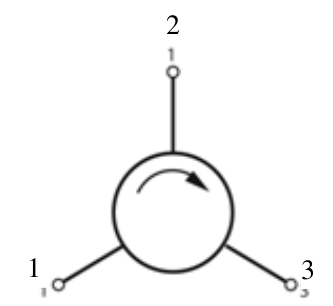
\includegraphics[width=4cm]{gfx/circulator.png}
 \caption{circulador de 3 puertos}
 \label{fig:circulator}
\end{figure}

La matriz de parámetros S es como sigue.

$$
\mathbf{S} = \begin{pmatrix} 0 & 0 & 1\\1 & 0 & 0\\0 & 1 & 0\end{pmatrix}
$$


\subsection{PSC}

El tipo de PSC modelado consiste en una red recíproca y adaptada en todos sus puertos, pero con pérdidas. Puede ser un 
componente de 3 o más puertos. A continuación se muestra la matriz de parámetros S genérica para una red de n puertos 
(matriz de nxn).

$$
\mathbf{S} = \begin{pmatrix} 0 & \dfrac{1}{n-1} & ... & \dfrac{1}{n-1}\\
							 \dfrac{1}{n-1} & 0 & ... & \dfrac{1}{n-1}\\
							 ... & ... & ... & ... \\
							 \dfrac{1}{n-1} & \dfrac{1}{n-1} & ... & 0 \end{pmatrix}
$$

\subsection{Acoplamientos mútuos}

El acoplamiento mútuo entre módulos radiantes es modelizado con el mismo comportamiento al de un cable, pero con las 
propiedades de atenuación y defasaje de una onda en el vacío. Las cuales son:

\begin{equation}
	S12 = S21 = \dfrac{e^{-jdfrac{\pi}{\lambda}r}}{4\pi r^2}
\end{equation}

siendo r la distancia recorrida por la señal. La matriz de parámetros S resulta,

$$
\mathbf{S} = \begin{pmatrix} 0 & \dfrac{e^{-jdfrac{\pi}{\lambda}r}}{4\pi r^2}\\\dfrac{e^{-jdfrac{\pi}{\lambda}r}}{4\pi r^2} & 0\end{pmatrix}
$$

\section{Ejemplo parámetros S}

En esta sección se ejemplifica el armado de las matrices de parámetros S de la antena desde el punto de transmisión a cada 
elemento radiante. Se asume que se tiene una antena de dos elementos radiantes con la configuración de RFDN de la figura 
\ref{fig:antennaS}.

\begin{figure}[H]
 \centering
 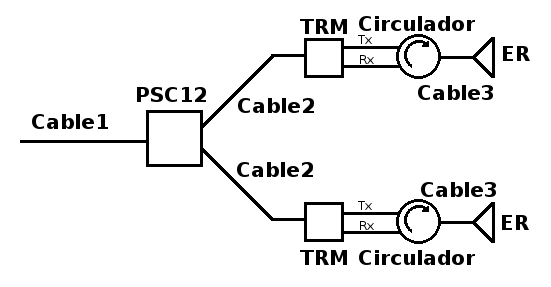
\includegraphics[width=9cm]{gfx/RFDN.png}
 \caption{RFDN del esquema de antena.}
 \label{fig:antennaS}
\end{figure}

La tabla \ref{tab:componentSParameters} muestra la cantidad de puertos que posee cada componente y la conexión de cada puerto.

\begin{table}[H]
  \footnotesize
  \centering
  \begin{tabular}{|c|c|p{6cm}|}
	\hline
	\textbf{Componente de Antena} & \textbf{Cantidad de puertos} & \textbf{Notas} \tabularnewline \hline 
	cable1 &  2 & \tabularnewline \hline
	\multirow{3}{*}{PSC12} & & Puerto1: conexión cable1 \tabularnewline
	 & 3 & Puerto2: conexión Cable2 (superior) \tabularnewline
	 & & puerto3: conexión Cable2 (inferior) \tabularnewline \hline
	Cable2 & 2 & \tabularnewline \hline 
	\multirow{3}{*}{TRM} & & Puerto1: conexión cable2 \tabularnewline
	 & 3 & puerto2: conexión Tx \tabularnewline 
	 & & puerto3: conexión Rx \tabularnewline \hline
	\multirow{3}{*}{Circulador} & & Puerto1: conexión Tx \tabularnewline
	 & 3 & puerto2: conexión Cable3 \tabularnewline 
	 & & puerto3: conexión Rx \tabularnewline \hline
	Cable3 & 2 & \tabularnewline \hline 
	RM & 1 & \tabularnewline \hline 
  \end{tabular}
  \caption{Propiedades físicas de cada componente de una antena}
  \label{tab:componentSParameters}
\end{table}

Para la obtención de la respuesta del sistema desde el punto de transmisión/recepción a cada elemento radiante se debe 
transformar las matrices de 3 puertos en matrices de 2 puertos. Para ello se debe determinar que puertos de conexión son los 
utilizados para la obtención de dicha matriz asumiendo que se desea obtener la respuesta del sistema de transmisión del 
elemento radiante 2 (camino en rojo de la figura \ref{fig:antennaSLoop}).

\begin{figure}[H]
 \centering
 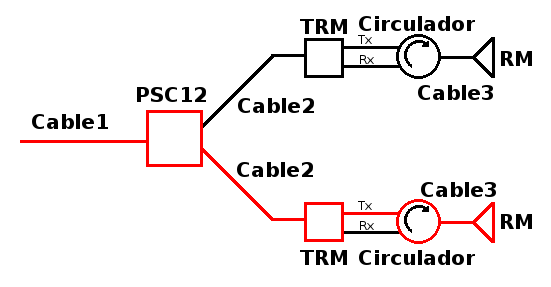
\includegraphics[width=9cm]{gfx/RFDNLoop.png}
 \caption{RFDN del esquema de antena. En rojo, cascada de redes de dos puertos.}
 \label{fig:antennaSLoop}
\end{figure}

Como los puertos utilizados por el PSC en el camino rojo de la figura \ref{fig:antennaSLoop} son el 1 y 3, la conversión de 
parámetros S resuta ser,

$$
	S_{PSC} = \begin{pmatrix} S11&S12&S13 \\ S21&S22&S23 \\ S31&S32&S33\end{pmatrix} \Rightarrow
	S_{PSC_{13}} = \begin{pmatrix} S11&S13 \\ S31&S33 \end{pmatrix}
$$

Los puertos utilizados por el TRM como el circulador son el 1 y 2, por lo tanto, la conversión de ambos parámetros S resulta 
equivalente.

$$
	S_{TRM} = \begin{pmatrix} S11&S12&S13 \\ S21&S22&S23 \\ S31&S32&S33\end{pmatrix} \Rightarrow
	S_{TRM_{12}} = \begin{pmatrix} S11&S12 \\ S21&S22 \end{pmatrix}
$$

$$
	S_{Circulador} = \begin{pmatrix} S11&S12&S13 \\ S21&S22&S23 \\ S31&S32&S33\end{pmatrix} \Rightarrow
	S_{Circulador_{12}} = \begin{pmatrix} S11&S12 \\ S21&S22 \end{pmatrix}
$$

Como se desea caracterizar la respuesta de una cascada de redes de dos puertos, se transforman todas las matrices de cada 
componente a parámetros T (ver equaciones \ref{eq:s2t}), se multiplican todas las matrices como se muestra en la ecuación 
\ref{eq:cascade} i luego, la matriz resultante se la vuelve a convertir a parámetros S (ver ecuaciones \ref{eq:t2s}).

$$
\begin{aligned}
	S_i &\Rightarrow T_i \\
	T_{in,rm2} &= T_{Cable1}T_{PSC_{13}}T_{Cable2}T_{TRM_{12}}T_{Circulador_{12}}T_{Cable3}T_{RM}\\
	T_{in,rm2} &\Rightarrow S_{in,rm2}
\end{aligned}
$$

Para el caso de querer caracterizar la respuesta inversa de la antena (desde el elemento radiante al receptor) del mismo camino 
mostrado en rojo de la figura \ref{fig:antennaSLoop}, el procedimiento es el mismo, salvo que se utilizan los puertos 2 y 3 del 
circulador y los puertos 1 y 3 del TRM.

$$
	S_{TRM} = \begin{pmatrix} S11&S12&S13 \\ S21&S22&S23 \\ S31&S32&S33\end{pmatrix} \Rightarrow
	S_{TRM_{13}} = \begin{pmatrix} S11&S13 \\ S31&S33 \end{pmatrix}
$$

$$
	S_{Circulador} = \begin{pmatrix} S11&S12&S13 \\ S21&S22&S23 \\ S31&S32&S33\end{pmatrix} \Rightarrow
	S_{Circulador_{23}} = \begin{pmatrix} S22&S23 \\ S32&S33 \end{pmatrix}
$$

Se vuelven a realizar los pasos de cascada de parámetros T y conversión a parámetros S de la matriz resultante. Pero, como 
dicho resultado sigue siendo desde el receptor al módulo radiante, se deben reacomodar los elementos de la matriz

$$
	S_{out,rm2} = \begin{pmatrix} S11&S12 \\ S21&S22\end{pmatrix} \Rightarrow 
	S_{rm2, out} = \begin{pmatrix} S22&S21 \\ S12&S11 \end{pmatrix}
$$

\todo{Hacer un montecarlo con todos TODOS los errores comunes, casi terminado, creo que esta, faltan los graficos}
\todo{Hacer un ensayo de cuanta diferencia es aceptable del conocimiento de la antena con cosas raras}

